%% Font size %%
\documentclass[11pt]{article}

%% Load the custom package
\usepackage{Mathdoc}
\usetikzlibrary{arrows.meta}

%% Numéro de séquence %% Titre de la séquence %%
\renewcommand{\centerhead}{Chap. 2 : Points, droites, segments}

%% Spacing commands %%
\renewcommand{\baselinestretch}{1}
\setlength{\parindent}{0pt}

\begin{document}

\section{Points}

\begin{definition}
  Un point est une position exacte du plan, sans dimension.
\end{definition}

\begin{notation}
  \begin{enuspaced}
  \item On le représente par une croix.
  \item On le nomme par une lettre \textbf{majuscule}.
  \end{enuspaced}
\end{notation}

\begin{exemple}
Trois points du plan : A, B et C. \\
\begin{tikzpicture}[scale=1]
  \tkzDefPoint(0,0){A}
  \tkzDefPoint(2.5,1){B}
  \tkzDefPoint(1.2,-0.6){C}
  \tkzDrawPoints[shape=cross out](A,B,C)
  \tkzLabelPoints(A,B,C)
\end{tikzpicture}
\end{exemple}

\section{Droites et demi-droites}

\begin{definition}
  Une droite est une infinité de points alignés, sans début ni fin.
\end{definition}

\begin{notation}
  Elle se note $(AB)$ (deux points qu'elle traverse) ou $(d)$ (une
  lettre minuscule). On la trace \textbf{à la règle}, avec une flèche
  à chaque bout.
\end{notation}

\begin{definition}
  Une demi-droite est une droite coupée en un point : son
  \textbf{origine}. Un seul côté continue à l'infini.
\end{definition}

\begin{notation}
  Elle se note $[AB)$ : $A$ est l'origine, la flèche est du côté de $B$.
\end{notation}

\begin{exemple}
Mêmes points $A$ et $B$, trois objets différents : \\ \\
\begin{center}
\begin{tabular}{ccc}
\begin{tikzpicture}[scale=0.9]
  \tkzDefPoint(0,0){A}
  \tkzDefPoint(2.5,0){B}
  \draw[thick] (A) -- (B);
  \tkzDrawPoints[shape=cross out](A,B)
  \tkzLabelPoints[below](A,B)
\end{tikzpicture}
&
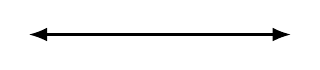
\begin{tikzpicture}[scale=0.9]
  \tkzDefPoint(0,0){A}
  \tkzDefPoint(2.5,0){B}
  \draw[thick,{Latex}-{Latex}] (-0.6,0) -- (3.1,0);
  \tkzDrawPoints[shape=cross out](A,B)
  \tkzLabelPoints[below](A,B)
\end{tikzpicture}
&
\begin{tikzpicture}[scale=0.9]
  \tkzDefPoint(0,0){A}
  \tkzDefPoint(2.5,0){B}
  \draw[thick,-{Latex}] (A) -- (3.1,0);
  \tkzDrawPoints[shape=cross out](A,B)
  \tkzLabelPoints[below](A,B)
\end{tikzpicture}
\\
Segment $[AB]$ & Droite $(AB)$ & Demi-droite $[AB)$
\end{tabular}
\end{center}
\end{exemple}

\section{Segments et appartenance}

\begin{definition}
  Un segment est la portion de droite comprise entre deux points $A$
  et $B$ : ses \textbf{extrémités}.
\end{definition}

\begin{notation}
  On le note $[AB]$ (ou $[BA]$), sa longueur se note $AB$. Pas de
  flèche : le trait s'arrête pile à $A$ et à $B$.
\end{notation}

\begin{exemple}
  Soit $[AB]$ un segment d'extrémités A et B : \\
      \input{.figures/segment1.txt}
\end{exemple}

\begin{definition}
  $C$ \textbf{appartient} au segment $[AB]$ si $C$ est situé entre
  $A$ et $B$, sur le segment. On note $C \in [AB]$. \\
  Sinon, on note $D \notin [AB]$.
\end{definition}

\begin{exemple}
  Soit $[AB]$ un segment, avec $C \in [AB]$ et $D \notin [AB]$ : \\
      \input{.figures/segment2.txt}
\end{exemple}

\section{Appartenance à une droite, à une demi-droite}

\begin{definition}
  $C$ appartient à une droite $(d)$ si $C$ est l'un des points de
  cette droite (n'importe où : la droite est infinie). On note $C \in (d)$.
\end{definition}

\begin{exemple}
  Ici, $C \in (d)$ : \\
\begin{tikzpicture}[scale=1.1]
  \tkzDefPoint(0,0){A}
  \tkzDefPoint(3,1.5){B}
  \tkzDefPoint(2,1){C}
  \draw[thick,{Latex}-{Latex}] (-0.9,-0.45) -- (3.9,1.95);
  \tkzDrawPoints[shape=cross out](C)
  \tkzLabelPoints[above](C)
  \tkzLabelSegment[sloped,below](A,B){$(d)$}
\end{tikzpicture}
\end{exemple}

\begin{remarque}
  Un point de la droite $(AB)$ n'appartient pas forcément à la
  demi-droite $[AB)$ !
\end{remarque}

\begin{exemple}
  Ici, $C \in (AB)$ mais $C \notin [AB)$ : \\
\begin{tikzpicture}[scale=1.1]
  \tkzDefPoint(0,0){A}
  \tkzDefPoint(2,1){B}
  \tkzDefPoint(-1,-0.5){C}
  \draw[thick,-{Latex}] (A) -- (3.6,1.8);
  \tkzDrawPoints[shape=cross out](A,B,C)
  \tkzLabelPoints[above](A,B,C)
  \tkzLabelSegment[sloped,below](A,B){$[AB)$}
\end{tikzpicture}
\end{exemple}

\section{Milieu d'un segment}

\begin{definition}
  Le milieu d'un segment $[AB]$ est le point $I$ qui vérifie :
  \begin{enu}
  \item $I \in [AB]$ ($I$ appartient au segment) ;
  \item $IA = IB$ ($I$ est à égale distance de $A$ et de $B$).
  \end{enu}
\end{definition}

\begin{exemple}
  Soit $I$ le milieu du segment $[AB]$ : \\
      \input{.figures/segment3.txt}
\end{exemple}

\end{document}

%%% Local Variables:
%%% mode: LaTeX
%%% TeX-master: t
%%% End:
